\documentclass[12pt]{article}
\usepackage{amsmath}
\usepackage{amsfonts}
\usepackage{tikz}
\usepackage{multicol}

\title{Introductory\\Sets Exercises\\
\begin{center}

\includegraphics[width=4em]{ApS_logo.png}
\end{center}
\begin{normalsize}Tutoring Centre Ferndale \end{normalsize}}
\author{}
\date{}
\begin{document}

\maketitle

\section*{Questions}

\begin{enumerate}
    % Notation and Definitions
    \item Define the following terms:
    \begin{enumerate}
        \item Set
        \item Element
        \item Subset
        \item Universal set
        \item Empty set
    \end{enumerate}
    
    \item Use set notation to write the set of all even numbers less than 20.

    \item Let \( A = \{1, 2, 3, 4\} \) and \( B = \{3, 4, 5, 6\} \). List the elements of \( A \cup B \).

    \item Let \( A = \{1, 2, 3, 4\} \) and \( B = \{3, 4, 5, 6\} \). List the elements of \( A \cap B \).

    \item Let \( A = \{1, 2, 3, 4\} \) and \( B = \{3, 4, 5, 6\} \). List the elements of \( A - B \).

    \item Let \( A = \{1, 2, 3, 4\} \) and \( B = \{3, 4, 5, 6\} \). List the elements of \( B - A \).

    \item Let \( A = \{x \mid x \text{ is a prime number less than 10} \} \). List the elements of \( A \).

    \item Let \( U = \{1, 2, 3, 4, 5, 6\} \) and \( A = \{1, 2, 3\} \). Find \( A' \) (the complement of \( A \)).

    \item Is \( \{1, 2\} \subseteq \{1, 2, 3, 4\} \)? Justify your answer.

    \item Is \( \{1, 2, 5\} \subseteq \{1, 2, 3, 4\} \)? Justify your answer.

    % Venn Diagrams
    \item Draw a Venn diagram to represent the sets \( A \) and \( B \) where \( A = \{1, 2, 3\} \) and \( B = \{3, 4, 5\} \).

    \item Using the Venn diagram from the previous question, shade the region representing \( A \cup B \).

    \item Using the Venn diagram from question 11, shade the region representing \( A \cap B \).

    \item Using the Venn diagram from question 11, shade the region representing \( A - B \).

    \item Using the Venn diagram from question 11, shade the region representing \( B - A \).

    % Theory and Application
    \item Explain the difference between a finite set and an infinite set, providing examples of each.

    \item Prove that the empty set is a subset of every set.

    \item If \( A \) and \( B \) are sets, prove that \( A \cap B \subseteq A \).

    \item If \( A \) and \( B \) are sets, prove that \( A \cap B \subseteq B \).

    \item Explain the significance of the universal set in set theory.

    % General Questions
    \item Given the sets \( A = \{2, 4, 6, 8\} \) and \( B = \{1, 2, 3, 4, 5\} \), find \( A \cup B \).

    \item Given the sets \( A = \{2, 4, 6, 8\} \) and \( B = \{1, 2, 3, 4, 5\} \), find \( A \cap B \).

    \item Given the sets \( A = \{2, 4, 6, 8\} \) and \( B = \{1, 2, 3, 4, 5\} \), find \( A - B \).

    \item Given the sets \( A = \{2, 4, 6, 8\} \) and \( B = \{1, 2, 3, 4, 5\} \), find \( B - A \).

    \item Let \( A = \{x \mid x \text{ is a vowel in the English alphabet} \} \). List the elements of \( A \).

    \item Let \( B = \{x \mid x \text{ is a consonant in the English alphabet} \} \). List the elements of \( B \).

    \item Determine if the following statement is true or false: \( \{x \mid x \text{ is a letter in the word 'book'}\} = \{b, o, k\} \).

    \item Determine if the following statement is true or false: \( \{x \mid x \text{ is a digit in the number 2024}\} = \{2, 0, 4\} \).

    \item Let \( A = \{x \mid x \text{ is a natural number less than 5} \} \). List the elements of \( A \).

    \item Let \( B = \{x \mid x \text{ is a natural number greater than 5 and less than 10} \} \). List the elements of \( B \).

    \item If \( A = \{1, 3, 5\} \) and \( B = \{2, 4, 6\} \), find \( A \cup B \).

    \item If \( A = \{1, 3, 5\} \) and \( B = \{2, 4, 6\} \), find \( A \cap B \).

    \item If \( A = \{1, 3, 5\} \) and \( B = \{2, 4, 6\} \), find \( A - B \).

    \item If \( A = \{1, 3, 5\} \) and \( B = \{2, 4, 6\} \), find \( B - A \).

    \item Let \( A = \{a, b, c, d\} \) and \( B = \{c, d, e, f\} \). Draw a Venn diagram and shade the region representing \( A \cup B \).

    \item Let \( A = \{a, b, c, d\} \) and \( B = \{c, d, e, f\} \). Draw a Venn diagram and shade the region representing \( A \cap B \).

    \item If \( U = \{1, 2, 3, 4, 5, 6, 7, 8\} \), \( A = \{2, 4, 6, 8\} \), and \( B = \{1, 2, 3, 4\} \), find \( (A \cup B)' \).

    \item If \( U = \{1, 2, 3, 4, 5, 6, 7, 8\} \), \( A = \{2, 4, 6, 8\} \), and \( B = \{1, 2, 3, 4\} \), find \( (A \cap B)' \).
\end{enumerate}

\newpage

\section*{Answers}

\begin{enumerate}
    % Notation and Definitions
    \item Definitions:
    \begin{enumerate}
        \item Set: A collection of distinct objects, considered as an object in its own right.
        \item Element: An object that is a member of a set.
        \item Subset: A set whose elements are all contained within another set.
        \item Universal set: The set that contains all the objects under consideration, usually denoted by \( U \).
        \item Empty set: A set with no elements, denoted by \( \emptyset \) or \( \{\} \).
    \end{enumerate}
    
    \item \(\{2, 4, 6, 8, 10, 12, 14, 16, 18\}\)

    \item \( A \cup B = \{1, 2, 3, 4, 5, 6\} \)

    \item \( A \cap B = \{3, 4\} \)

    \item \( A - B = \{1, 2\} \)

    \item \( B - A = \{5, 6\} \)

    \item \( A = \{2, 3, 5, 7\} \)

    \item \( A' = \{4, 5, 6\} \)

    \item Yes, because every element of \(\{1, 2\}\) is also in \(\{1, 2, 3, 4\}\).

    \item No, because 5 is not in \(\{1, 2, 3, 4\}\).

    % Venn Diagrams
    \item \begin{center}
        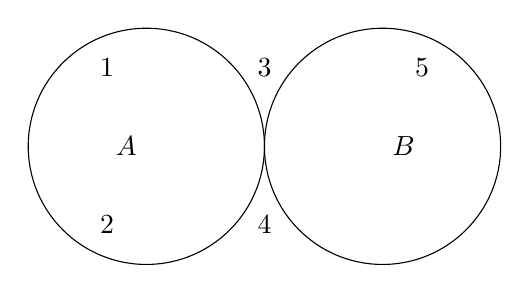
\begin{tikzpicture}
            \begin{scope}
                \clip (-1.5,0) circle (1.5);
                \fill[gray] (1.5,0) circle (1.5);
            \end{scope}
            \draw (-1.5,0) circle (1.5) node [left] {$A$};
            \draw (1.5,0) circle (1.5) node [right] {$B$};
            \node at (-2,1) {1};
            \node at (0,1) {3};
            \node at (0,-1) {4};
            \node at (2,1) {5};
            \node at (-2,-1) {2};
        \end{tikzpicture}
    \end{center}

    \item \begin{center}
        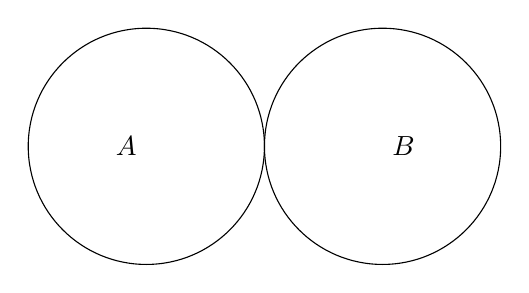
\begin{tikzpicture}
            \begin{scope}
                \clip (-1.5,0) circle (1.5);
                \fill[gray] (1.5,0) circle (1.5);
            \end{scope}
            \draw (-1.5,0) circle (1.5) node [left] {$A$};
            \draw (1.5,0) circle (1.5) node [right] {$B$};
        \end{tikzpicture}
    \end{center}

    \item \begin{center}
        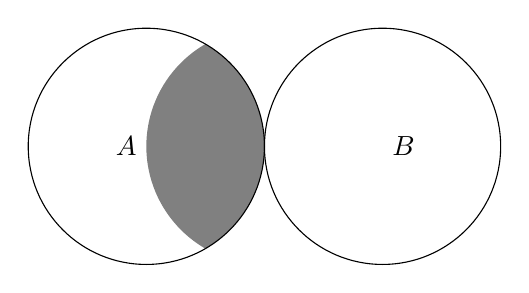
\begin{tikzpicture}
            \begin{scope}
                \clip (-1.5,0) circle (1.5);
                \fill[gray] (0,0) circle (1.5);
            \end{scope}
            \draw (-1.5,0) circle (1.5) node [left] {$A$};
            \draw (1.5,0) circle (1.5) node [right] {$B$};
        \end{tikzpicture}
    \end{center}

    \item \begin{center}
        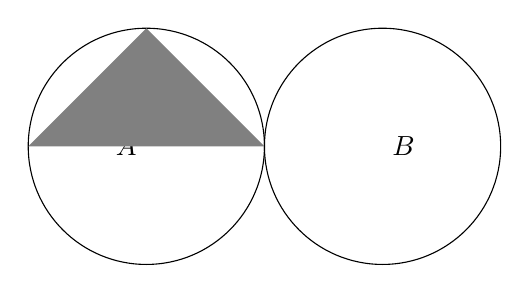
\begin{tikzpicture}
            \draw (-1.5,0) circle (1.5) node [left] {$A$};
            \draw (1.5,0) circle (1.5) node [right] {$B$};
            \begin{scope}
                \clip (-1.5,0) circle (1.5);
                \fill[gray] (-3,0) -- (0,0) -- (-1.5,1.5) -- cycle;
            \end{scope}
        \end{tikzpicture}
    \end{center}

    \item \begin{center}
        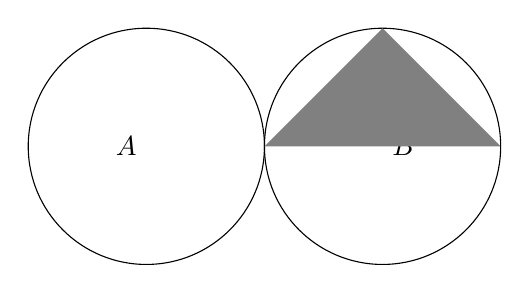
\begin{tikzpicture}
            \draw (-1.5,0) circle (1.5) node [left] {$A$};
            \draw (1.5,0) circle (1.5) node [right] {$B$};
            \begin{scope}
                \clip (1.5,0) circle (1.5);
                \fill[gray] (0,0) -- (3,0) -- (1.5,1.5) -- cycle;
            \end{scope}
        \end{tikzpicture}
    \end{center}

    % Theory and Application
    \item A finite set has a limited number of elements, e.g., \(\{1, 2, 3\}\). An infinite set has unlimited elements, e.g., \(\{1, 2, 3, \ldots\}\).

    \item Proof: Let \( A \) be any set. The empty set \( \emptyset \) has no elements. For any element \( x \in \emptyset \), \( x \in A \) is vacuously true. Hence, \( \emptyset \subseteq A \).

    \item Proof: If \( x \in A \cap B \), then \( x \in A \) and \( x \in B \). Therefore, \( x \in A \), so \( A \cap B \subseteq A \).

    \item Proof: If \( x \in A \cap B \), then \( x \in A \) and \( x \in B \). Therefore, \( x \in B \), so \( A \cap B \subseteq B \).

    \item The universal set \( U \) encompasses all objects under consideration, providing a context for defining complements and other set operations.

    % General Questions
    \item \( A \cup B = \{1, 2, 3, 4, 5, 6, 8\} \)

    \item \( A \cap B = \{2, 4\} \)

    \item \( A - B = \{6, 8\} \)

    \item \( B - A = \{1, 3, 5\} \)

    \item \( A = \{a, e, i, o, u\} \)

    \item \( B = \{b, c, d, f, g, h, j, k, l, m, n, p, q, r, s, t, v, w, x, y, z\} \)

    \item True, because the set of letters in 'book' is \(\{b, o, k\}\).

    \item True, because the set of digits in 2024 is \(\{2, 0, 4\}\).

    \item \( A = \{1, 2, 3, 4\} \)

    \item \( B = \{6, 7, 8, 9\} \)

    \item \( A \cup B = \{1, 2, 3, 5\} \)

    \item \( A \cap B = \emptyset \)

    \item \( A - B = \{1, 3, 5\} \)

    \item \( B - A = \{2, 4, 6\} \)

    \item \begin{center}
        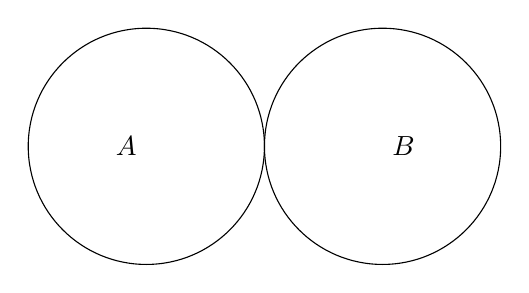
\begin{tikzpicture}
            \begin{scope}
                \clip (-1.5,0) circle (1.5);
                \fill[gray] (1.5,0) circle (1.5);
            \end{scope}
            \draw (-1.5,0) circle (1.5) node [left] {$A$};
            \draw (1.5,0) circle (1.5) node [right] {$B$};
        \end{tikzpicture}
    \end{center}

    \item \begin{center}
        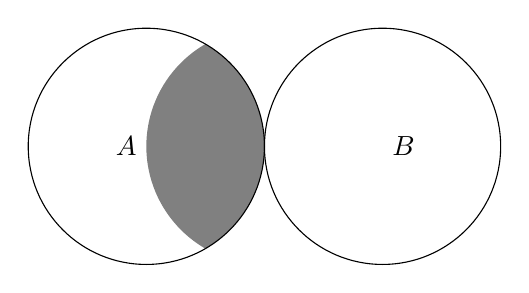
\begin{tikzpicture}
            \begin{scope}
                \clip (-1.5,0) circle (1.5);
                \fill[gray] (0,0) circle (1.5);
            \end{scope}
            \draw (-1.5,0) circle (1.5) node [left] {$A$};
            \draw (1.5,0) circle (1.5) node [right] {$B$};
        \end{tikzpicture}
    \end{center}

    \item \( (A \cup B)' = \{7, 8\} \)

    \item \( (A \cap B)' = \{1, 3, 5, 7, 8\} \)
\end{enumerate}

\end{document}
